Assuming $r_0 = (1, -1)$, what is the initial gradient at $r_0$? What would be a reasonable choice for $\lambda_0$ so that $r_1$ is not too far from the continuous path? Plot $r_1$ on your contour plot.

\begin{solution}
\begin{align*}
    \nabla f(1, -1) = \begin{bmatrix}
        -5 \\ 1
    \end{bmatrix}
\end{align*}

A $\lambda$ value of $0.1$ keeps the $r_1$ value close to the continuous path.

\begin{center}
    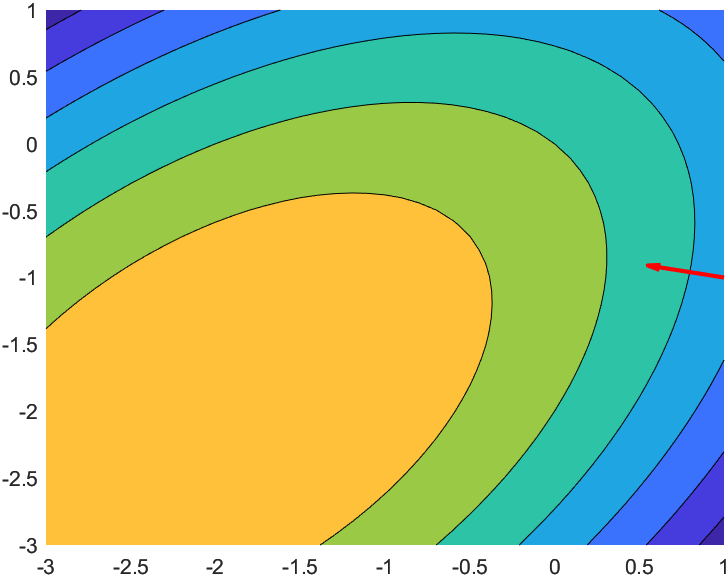
\includegraphics[width=0.5\textwidth]{img/e7p4.png}
\end{center}
\end{solution}